%!TEX ROOT = thesis.tex
\chapter{Framework Overview}

\section{Introduction}
In order to tackle the issues identified through the research questions and literature review, the theoretical framework is laid as to provide a conceptual schema on how to break the rather huge and intricate challenge into multiple bite sized puzzles. First, the overview of the proposed framework used in this work is described in Section \ref{section:framework}. Next, the description of the dataset used is described in Section \ref{section:dataset_used} and finally, this chapter concludes with the experimental methodology applied in this work to obtain the published results (see Section \ref{sec:expmethodology}). 



\section{Framework Overview}
\label{section:framework}
In this section, a high level overview of the fundamental processing step along with two suggested core components for vehicle semantic extraction and retrieval is provided. The groundwork described in this work abides to the typical top-down approach used in Intelligent Transportation System (ITS) where the video data is subjected to background subtraction, followed by blob filtering, vehicle detection as well as vehicle tracking is as described in \cite{lim2017}. The semantic information from the vehicle blobs are then extracted and stored in the database. 

Now, with the vehicle specific semantics stored in the database, retrieval engines were designed to enabled users to easily retrieve the stored information. Both retrieval engines features a graphical user interface which allows users to enter the queries by drawing the desired trajectory on the search interface as well as providing other crucial information which would assist in identifying the targeted video shot.


\begin{figure}[hbt!]\centering
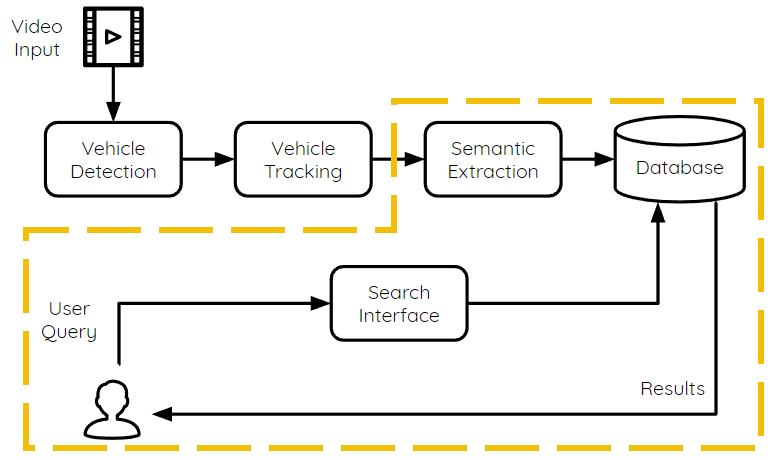
\includegraphics[width=.9\textwidth]{image/new/framework_new.PNG}
\caption{Framework Diagram, Contribution in Highlighted Border}
\label{fig:framework}
\end{figure}


In this work, two frameworks were suggested and used for the vehicle semantic extraction and retrieval process. Both frameworks utilise an underlying distinctive approach, with the same end goal in mind, which is the retrieval of desired video snippets which closely resembles a user described query. For each of these frameworks, the formulation of idea, steps and process involved are described in this chapter. 
%As there are various solutions proposed in this work, solutions which are common to both core frameworks is also provided. 
As a whole, the end-to-end framework can be visualised using Figure \ref{fig:framework} where the main contribution of this work is highlighted in yellow border. 

\subsection{LSH-Inspired Retrieval Framework}
The first of the two frameworks suggested in this work is the \textit{LSH-Inspired Retrieval Framework}. Locality-Sensitive Hashing (LSH) is a technique used for dimensionality reduction, typically to perform hashing on a set of documents so that documents with similar properties are mapped and clustered to similar locality or neighbourhood. This technique excels especially when working with high dimensional data such as video data.

Inspirations to cluster similar documents were drawn from the LSH technique and implemented in this framework. The extracted semantics from each vehicle blobs were clustered into semantic groups which contains colour and motion information. This concept was adopted in the proposed method with the following considerations in mind: 

\begin{enumerate}
    \item Ease of Interpretation \& Access: As the extracted semantics are stored in clusters of similar properties, these semantics can be easily interpreted and retrieved. 
    \item Reduction of Input/Output (I/O) Bottleneck: As the proposed method stores the extracted semantics in a database, I/O bottlenecks are bound to occur when reading and retrieving large quantity of data. As the semantics of similar properties are clustered together, the retrieval engine does not have to search through the entire set of database for records that matches the given query.
\end{enumerate}


\subsection{Chamfer Distance-Inspired Framework}
The second of the two frameworks suggested in this work is the \textit{Chamfer Distance-Inspired Framework}. Chamfer distance is one of the many distance measure (see Section \ref{section:distancemeasures}) introduced by mathematicians and researchers. Chamfer Distance, as introduced by \cite{barrow1977parametric}, was originally designed to match images by comparing the shapes of two collections of shape fragments. However, in this framework, the use of chamfer distance was modified to suite the research problem of comparing the shapes of vehicle trajectories. While the implementation of chamfer distance measure in this framework has its advantages, it also comes with some drawbacks. The considerations taken when designing this frameworks are as such:


\begin{enumerate}
    \item The use of Chamfer Distance to compare trajectories allows the retrieval engine to search from a wider range, however, this comes with extra computational cost. While the disadvantages were undesirable, the benefits outweighs this drawback by providing a higher recall rate for the retrieved results. Along with that, the use of time and date filtering could potentially reduce the number of records, hence, further reducing the computational cost. 
    \item The ranking of results is a desirable feature in a retrieval engine. As Chamfer Distance produces a distance score for every pair of trajectories compared, this score can be used to sort the results in an intuitive manner where results of higher resemblance would appear higher in the ranking.  
\end{enumerate}


\section{Dataset}
\label{section:dataset_used}

In view of testing the proposed framework for large-scale extraction and retrieval of video semantics, a new collection of video dataset was gathered. A stationary cloud-enabled web camera was set up on the fourth floor of a building with a window facing a piece of private car park area. Figure \ref{fig:camerasetup} depicts the camera setup overcasting the car park area. 

The aforementioned setup was done to mimic a typical camera setup which tower over a piece of outdoor car park lot that are found in the wild. 


\begin{figure}[hbt!]\centering
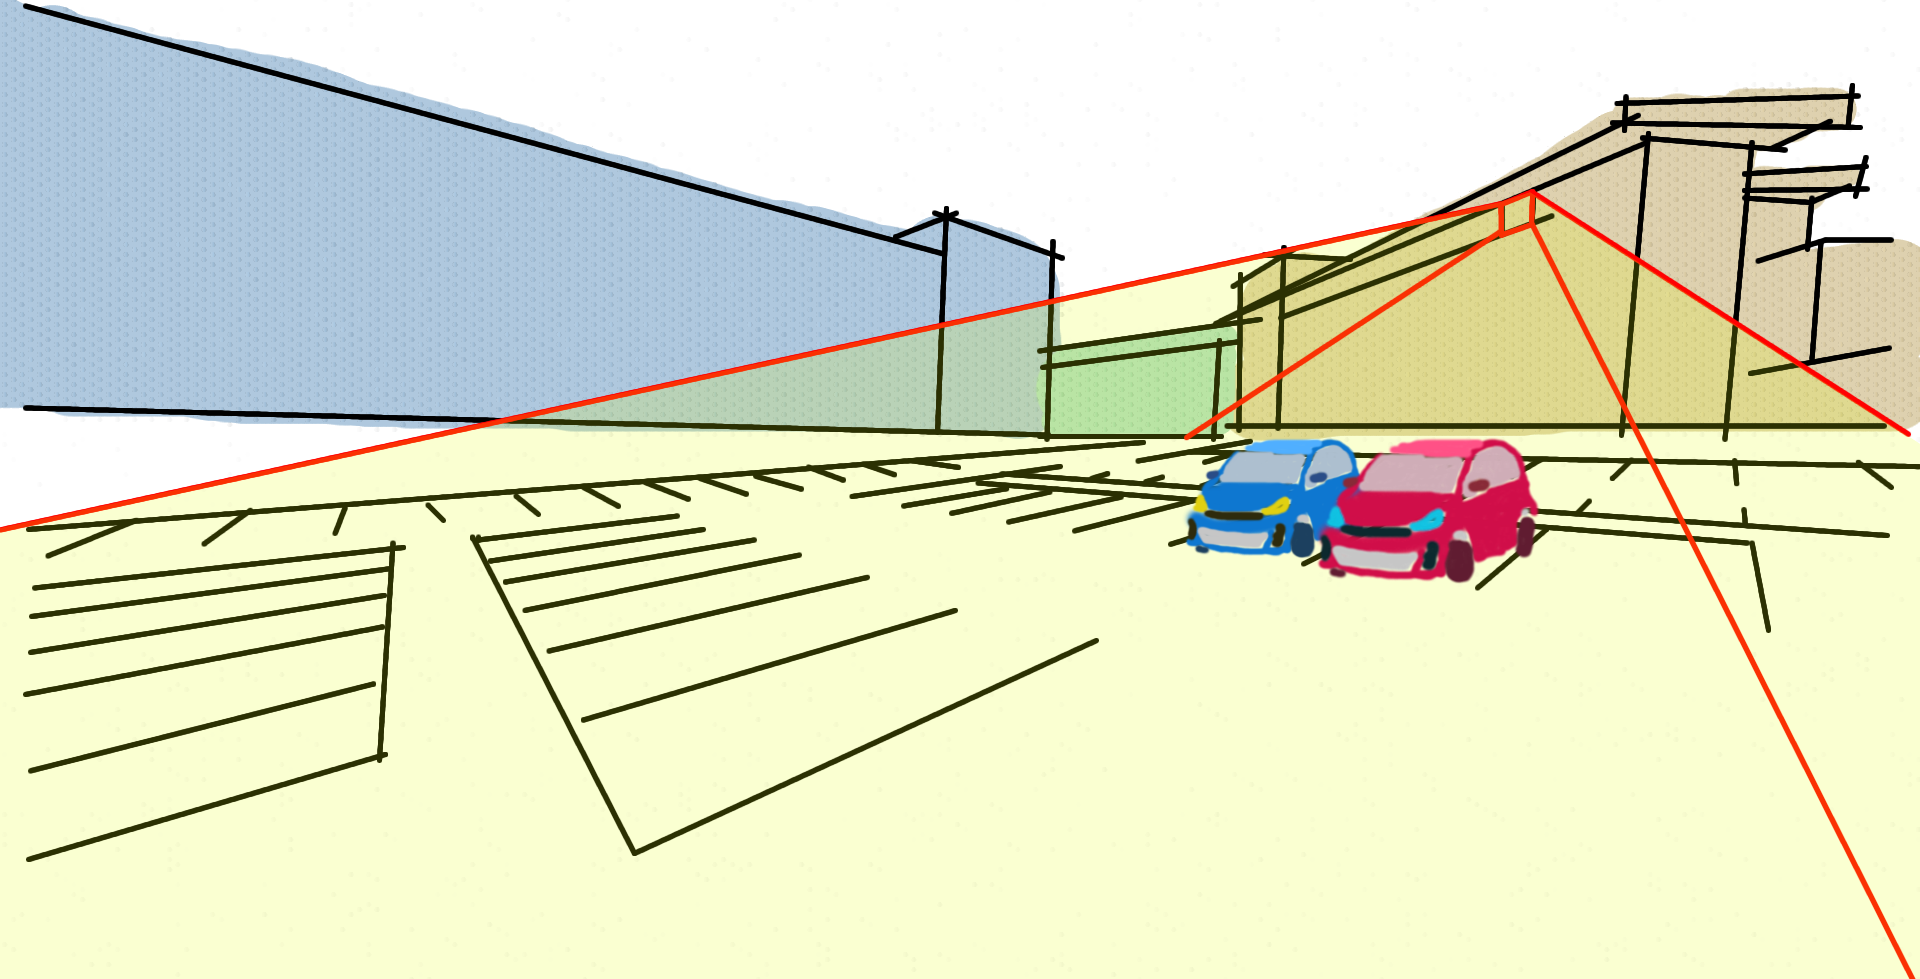
\includegraphics[width=.8\textwidth]{image/new/fcicarpark2.png}
\caption{Camera setup to capture the car park from the fourth floor}
\label{fig:camerasetup}
\end{figure}


\begin{figure}[!hbt]\centering
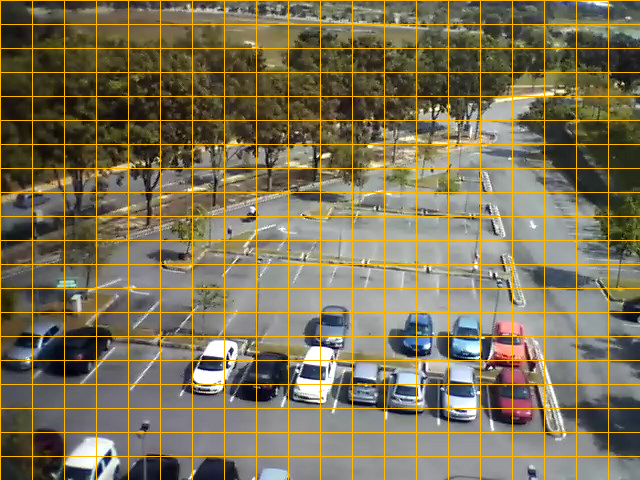
\includegraphics[width=.7\textwidth]{image/general/grids.png}
\caption{View from camera setup; 20$\times$20 Grids}
\label{fig:viewfromcamera}
\end{figure}


Through the camera's web interface, this device was set to record on weekdays from Monday through Friday, starting from 08:30 in the morning up until 18:30 in the evening, with a total of 10 hours of video being recorded each day. Among the important settings, each recorded video clip was set to have a maximum length of 6 minutes, and hence, 10 video clips every hour, and a total of 100 at the end of each day. The recorded video clips were saved into the external microSD memory card. At the end of each day, the data was then copied over to a server via a script. However, due to glitches that occurred during the recording process, some of the video clips were cut off abruptly. Hence, some of the days do not contain the full 10 hours video clips. 

\begin{table}[!ht]\centering
\begin{tabular}{ll}
Camera Model: & Dlink DSC-942L        \\
Resolution:   & 640$\times$480 pixels \\
Frame rate:   & 10 $fps$             \\
Format:       & H.264 / MPEG-4 AVC    \\
Naming Convention: & $CCYYMMDD\_HHMMSS.mp4$
\end{tabular}
\vspace{1em}
\caption{Details of the Camera Setup used for Data Collection}
\end{table}

\begin{figure}[!htb]
  \centering

\begin{tabular}{cc}
 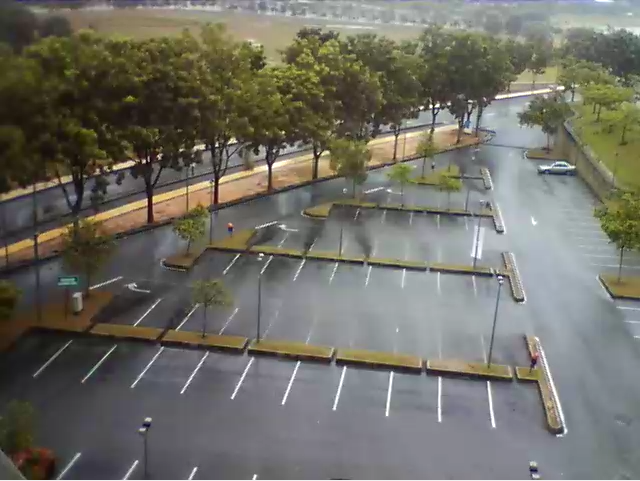
\includegraphics[width=0.4\linewidth]{image/general/rain.PNG} &  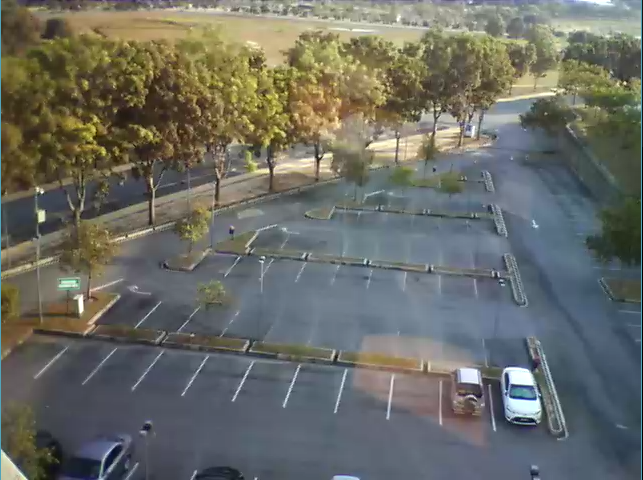
\includegraphics[width=0.4\linewidth]{image/general/reflection.PNG}\\ 
\begin{tabular}{c}(a) Rainy day with \\ reflective surface\end{tabular} & \begin{tabular}{c}(b) Reflection on the \\car park from the window\end{tabular} \\
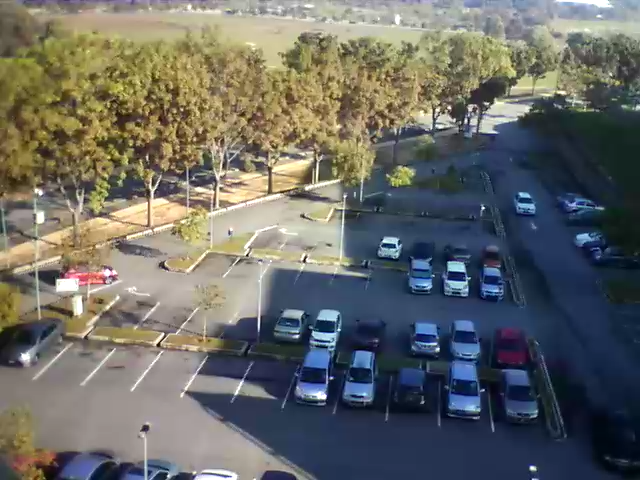
\includegraphics[width=0.4\linewidth]{image/general/shadow.png} &  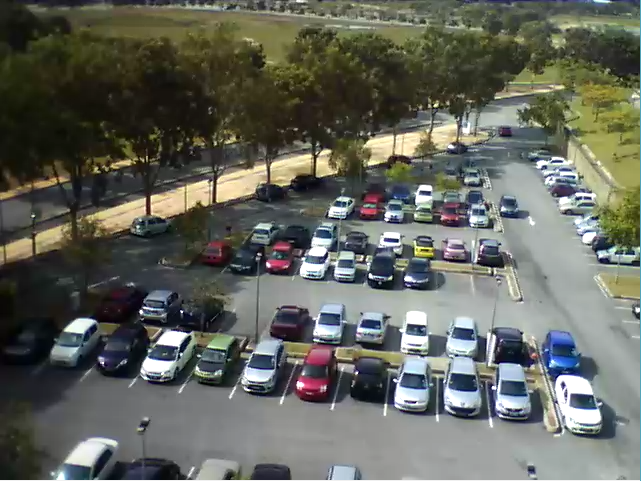
\includegraphics[width=0.4\linewidth]{image/general/shadow2.png}\\
\begin{tabular}{c}(c) Severe shadow over \\ the car park (08:48AM)\end{tabular} & \begin{tabular}{c}(d)  Severe shadow over \\ the car park (04:06PM)\end{tabular}
\end{tabular}


\caption{Noisy Data Within the Collected Dataset} \label{fig:weather}
\end{figure}


This setup was left to record data over the course of several months with various weather conditions, lighting conditions as well as a diverse set of car park scenes which includes peak hours with plenty of vehicles along with the off-days. In addition to that, this setup covers a total of over 45 parking lots which excludes parking lots that are too small or occluded. Figure \ref{fig:weather} exhibits the various weather conditions and noise which were recorded sporadically throughout the dataset.





\section{Experimental Methodology}
\label{sec:expmethodology}

In the subsequent chapters, the detailed descriptions of the proposed vehicle semantic extraction algorithm as well as the retrieval engine modules will be provided. In this section, the methodology and the experimental setup is briefly discussed to provide an overview on how the experiments will be performed in this work.

As the performance of the proposed method is essential towards end users, each of the proposed algorithm in the framework is evaluated with the help of volunteers. Even though the fundamental framework was adopted from \cite{lim2017} without changes on the underlying algorithm, errors which were propagated from the Vehicle Detection and Vehicle Tracking modules were not overlooked nor discarded during the evaluation of the subsequent modules in the pipeline. This was done intentionally to provide an end-to-end assessment of the framework. 

The proposed methods were implemented and evaluated on an Intel i7 machine with 16GB RAM, GeForce GTX 1060 GPU. As the main focal point in this proposed method revolves around the semantic extraction of \textbf{vehicle colour} along with the \textbf{vehicle trajectory}, both of these components were assessed and evaluated individually to better understand the performance, effectiveness as well as the weakness of the proposed methods. This, in turn, provides a deeper understanding and opportunities for improvements as well as future works. 

Two retrieval engines were designed and implemented in this work, the objective of the first retrieval engine was to build a prototype for the evaluation of the its current performance and to identify gaps to be improved. This process allowed the author to return to the drawing board and reevaluate the algorithms, metrics and evaluation process performed. Given this setup, the experimental methodology can be divided into two phase. Given that the data were fully annotated, the evaluation metrics used for Phase One experiment was Accuracy, Recall, and $F_1$ Score.


\subsection{Phase One - Prototype}
While the collected dataset comprised of several months of data, only two days of data (20 hours) were used for the evaluation of \versionOneRet. Several annotators were deployed to manually label and fully annotate these data. Upon completing the annotation process, the annotators would cross-check to verify the sanctity of the annotation, along with that, the cross-checking allows the annotators to arrive at consensus on annotations that did not tally. The annotators were asked to take note of following events:
\begin{enumerate}
    \item Number of vehicle of each colour category (11 categories, see \ref{table:colorshex})
    \item Number of vehicles performing motion $TQ1$ \& $TQ2$ (See Figure \ref{fig:versionOneInterface})
\end{enumerate}



\subsection{Phase Two - Full Experiment}

During the Phase One of the experiment, it was noted that the entire annotation process was taking up a significant amount of work despite only using two days of data. As one month of data was set aside for the evaluation of the \versionTwoRet, an alternative methodology was applied. Typically, with any retrieval engine of all intents and purposes dealing with long-term data, it is not feasible to annotate a huge amount of ground truth manually as it is a labour intensive, mundane and time consuming process. Hence in this phase, one month of data was processed and evaluated without the manual annotations of all the events. 
%Instead, the best practice used in evaluating a large scale retrieval engine was used to document the evaluation process. 

Given that the final output of this work is a end-user facing retrieval system, the evaluation process took on an empirical user study approach. This unbiased approach provided users with full control and freedom to perform any kinds of search, and provide feedback for each of the result.
With this setup, a group of six volunteers were tasked to perform queries on the retrieval system for both the colour and trajectory of the vehicles and provide relevance score for each retrieved results. 
As the data in Phase Two was not fully annotated, it is impossible to compute the Recall and $F_1$ score. Instead, the Precision@K along with the normalised Discounted Cumulative Gain (nDCG) metrics were used. 

